\documentclass{article}
\bibliographystyle{alpha}
\usepackage{amsmath}
\usepackage{amssymb}
\usepackage{amsthm}
\usepackage{textcomp}
\usepackage{graphicx}

\author{Aditya Modi}
\title{CS252 Assignment Report}
\date{\today}

\begin{document}

\maketitle

\section{Introduction}
This assignment is given as a recap to the prequel course CS251.

\section{Assignment}

\subsection{Phase 1}
\label{octave}
Octave code generates random set of students with marks over 3 courses. Uniqueness is maintained by choosing a subset fro permutation of a set.
\subsection{Phase 2}
\label{p2}
A perl script is written to make a MySQL database of following form\\

\begin{table}[!htpb]
	\label{tab:marks}
	\begin{center}
		\begin{tabular}{|c|c|c|c|c|}
		\hline
		roll & course & assignment & project & exam \\
		\hline
		\end{tabular}
	\end{center}
	\caption{marks}
\end{table}

Similarly names table is to be created.

\begin{table}[!htpb]
	\label{tab:names}
	\begin{center}
		\begin{tabular}{|c|c|}
		\hline
		roll & name \\
		\hline
		\end{tabular}
	\end{center}
	\caption{names}
\end{table}

\subsection{Phase 3}
Using Table~\ref{tab:marks} and Table~\ref{tab:names} created in section~\ref{p2} by adding two columns \emph{total} and \emph{grade} on following basis.

\begin{equation*}
	\label{eq:grade}
		grade = 
		\begin{cases}
			A* & \text{if} \quad total \leq 95\%,\\
			A & \text{if} \quad 80\% \leq total < 95\%,\\
			A & \text{if} \quad 60\% \leq total < 80\%,\\
			A & \text{if} \quad 45\% \leq total < 60\%,\\
			A & \text{if} \quad 30\% \leq total < 45\%,\\
			A & \text{if} \quad total < 30\%.\\
		\end{cases}
\end{equation*}

\subsection{Phase 5}
Have to create a gnuplot cluster histogram.

\begin{figure}[!htpb]
	\label{fig:p5}
	\begin{center}
		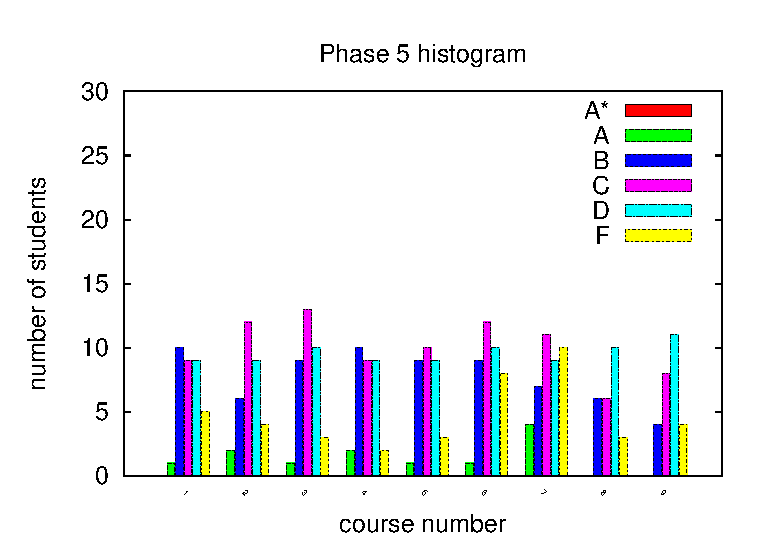
\includegraphics[width=0.6\columnwidth,height=0.5\columnwidth,keepaspectratio]{phase5.eps}
	\end{center}
	\caption{Phase 5 histogram}
\end{figure}

\subsection{Phase 6}
Created this file.

\subsection{Phase 7}
Created bash script for sorting and finding rank of students.

\subsection{Phase 8}
Link all files by creating a bash script to solve the assignment.

\section{Result}
No use of the assignment.

\bibliography{phase6}

\end{document}